\ifdefined\BuildingFromMainFile
\else
   \documentclass[../main.tex]{subfiles}
   \begin{document}
\fi


\graphicspath{{figure/}{../figure/}}

\newpage
\onehalfspacing

\linespread{1.25}
\setlength{\parskip}{\baselineskip}

\normalsize

\section{Genomic technologies to assess genetic variations in livestock}

Cattle is an important livestock species capable of converting low-quality and human-inedible proteins into high-quality proteins. The global cattle population is highly diverse due to intense selection for specific breeding goals, such as production of milk, beef, or both (dual-purpose), as well as the adaptation to a wide range of environments \citep{zhang2020evolution}. Due to selective breeding and improved husbandry conditions, spectacular increases in livestock productivity have been achieved. For example, the average annual milk yield per cow in the United States of America has increased by more than five-fold from 1,890 kg in 1924 to 9,682 kg in 2011 \citep{georges2019harnessing}. 

Genomic selection had been proposed to further accelerate genetic gain \citep{meuwissen2001prediction}. To this end, the genetic value of an individual is predicted based on genome-wide molecular marker information. Genotyping arrays were developed to assess variation at thousands of polymorphic sites in the cattle genome. The genotype information is then linked to phenotype either to determine markers associated with agriculturally-important traits \citep{goddard2009mapping} or to derive the prediction equation for genomic selection \citep{meuwissen2001prediction}. More than 3 million cattle in the USA have already been genotyped \citep{wiggans2017genomic}. However, variations interrogated by chip-based genotyping  are  not comprehensive enough  to pinpoint causal mutations underlying the traits \citep{pausch2017evaluation}.

This limitation prompted the widespread utilization of whole-genome short-read sequencing. In this approach, the DNA is first fragmented and subsequently read in segments of few hundred bases (Fig. \ref{fig11:reseq}). Variation discovery typically follows a reference-guided alignment approach. Genotypes are called at positions where the observed nucleotides from the alignments differ from the corresponding reference nucleotides. Sophisticated variant calling algorithms were developed to differentiate between real variants and sequencing errors from noisy short-read data or misalignments \citep{depristo2011framework}. Whole genome sequencing approaches can accurately discover small variants (SNPs and Indels < 50 bp) across the whole genome. 

Sequencing costs have dropped substantially over the past decades, faster than Moore’s Law (a term in computer hardware that doubling power every two years indicates a well-progressed technology), which has paved the way towards sequencing a gigabase-sized genome for only \$100 \citep{Regalado2020,Wetterstrand2020}. The decline in sequencing costs has also enabled the sequencing of individual cattle genomes for agricultural applications. The 1000 Bull Genomes Project was launched to coordinate global sequencing efforts and compile huge datasets.  In their latest  (8$^{th}$ ) run, the consortium has already catalogued more than 150 million variants from more than 4000 cattle across 200 breeds \citep{hayes20191000}. This variant database has become a powerful resource to impute sequence variant genotypes into large mapping cohorts, thus accelerating the discovery of causal mutations for complex and monogenic traits, and improve the prediction accuracy of genomic selection \citep{daetwyler2014whole}. Recently, low-pass sequencing (<1x) coupled with genotype imputation were proposed as a cost-effective strategy to enable population-scale whole genome sequencing variant analysis \citep{snelling2020assessment}. \\

\bigskip

\begin{figure}[!htb]
    \centering
    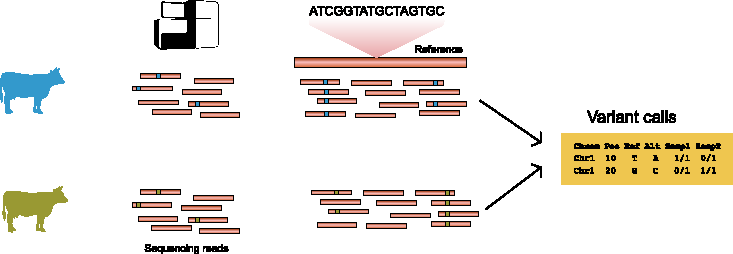
\includegraphics[width=\textwidth]{intro/fig1.pdf}
        \vspace{3mm}
        \caption[Identification of genetic variants through genome sequencing]{\textbf{Identification of genetic variants through re-sequencing} \\
        \footnotesize{The DNA of individual animals are fragmented into billions of short fragments which are then read by DNA sequencer in a massively parallel manner. Subsequently, the sequencing reads are compared (aligned) to the reference genome. Genetic variants are identified as nucleotide discordances relative to the reference sequences.}}
        \label{fig11:reseq}
\end{figure}


\section{Improvements in the cattle reference genome} 

A well-annotated reference genome is the starting point for many genomic analyses. It serves as a reference point for read alignment, variant calling, gene annotation, and functional analysis. Gene loci are defined at specific genomic coordinates, and alleles are referred to as alternative or reference  nucleotides. The ability to compare billions of sequencing reads from hundreds to thousands of individuals to reference sequences has quickly become the gold standard, identifying variants underpinning  inherited diseases or other relevant traits, thus accelerating genetic progress \citep{bickhart2020symposium}.

The first cattle reference genome (Btau 3.1 and Btau 4.0) was assembled in 2009 from bacterial artificial chromosome (BAC) and whole-genome shotgun (WGS) sequencing \citep{elsik2009genome}. The contig and scaffold N50 (i.e., 50\% of the genome is in contigs of this size or greater) for this assembly were 48.7 kb and 1.9 Mb respectively. This assembly was further refined in 2014 to close gaps and correct structural errors (UMD\_3.1.1) using additional sequencing data and sophisticated assembly approaches \citep{zimin2009whole}. The most recent cattle reference genome (ARS-UCD 1.2) was assembled using single-molecule real-time (SMRT) long-read sequencing data and scaffolded with optical mapping data. The quality of the resulting assembly improved considerably over UMD3.1 with contig and scaffold N50 values of 25.89 Mb and 103 Mb, respectively \citep{rosen2020novo}. Advances in assembly techniques (e.g., trio binning) and the development of highly accurate long-read sequencing technology now enable constructing assemblies of high continuity, correctness and completeness \citep{bickhart2020symposium}. The recently generated bovine assemblies exceed in quality the current \emph{Bos taurus} reference genome with contig N50 larger than 70 Mb and could resolve complex genomic regions, e.g. major histocompatibility regions \citep{rice2020continuous}. Trio binning takes advantage of the high heterozygosity in hybrids to separate long reads according to parental origins. The assembly is subsequently performed separately from the partitioned reads resulting in two haplotype-resolved assemblies. This approach  was first applied  to a cross between \emph{Bos taurus} x \emph{Bos indicus} cattle (Angus x Brahman) \citep{koren2018novo}, but now has been applied to broad range cattle breeds, including  undomesticated and/or cattle relatives (yak, gaur, bison) \citep{oppenheimer2021reference}. Recently, the Bovine Pangenome Consortium \citep{heaton2021reference} was initiated to coordinate genome assembly efforts and characterize the complete diversity from hundreds of global cattle breeds, including their wild-relatives and under-represented breeds. 

\section{One reference genome is not enough}

\subsection*{A single linear genome cannot fully represent species diversity}

Despite recent spectacular quality improvements, linear reference genomes are unable to represent the full genomic diversity within a species. A linear reference genome typically represents a mosaic haplotype assembled from either one or a few individuals. For example, the current cattle reference genome (ARS-UCD1.2) was assembled from a DNA sample from a single highly-inbred animal from the Hereford breed named Dominette, which was initially selected to simplify the assembly process \citep{rosen2020novo}. Reference assemblies from  other livestock species were generated using a similar approch, e.g., Duroc breed used for Sscrofa11.1 pig reference \citep{warr2020improved}, San Clemente breed for domestic goat reference \citep{bickhart2017single}, and Boxer breed for  CanFam 3.1 dog reference \citep{lindblad2005genome}. While the selection of reference animals seems to be a trivial process, the resulting reference sequences do not necessarily reflect the most common alleles that segregate in the population or from samples with breed-defining phenotypes \citep{ballouz2019time}. Reference-guided variant discovery might reflect some properties of the reference animal rather than the population; e.g., variant calling will discover more variants when the reference  contains rare alleles. \citet{Low2020} found a striking difference in the number of polymorphic sites when calling Angus variants from an Angus reference than from a Brahman reference. Additionally, the reference genome might carry the lower frequency variants or variants private to the reference animals. \citet{shukla2019hg19kindel} and \citet{ballouz2019time} estimated that 2 million bases in the human reference genome are minor alleles. 

\subsection*{Insufficient representation of genetic diversity by linear genomes cause reference bias}

Because alignment algorithms compare the reads towards the reference and try to minimize differences, the reference-guided variant discovery is biased towards the reference bases. In other words, it is easier to align DNA fragments without differences to the reference bases than DNA fragments  that contain non-reference bases. Comparison of the sequencing reads with variants, even if they are the true representation of that species, will be penalized, resulting in sub-optimal alignments, misalignments, or unmapped reads (Fig. \ref{fig12:bias}) \citep{pritt2018forge}. Together, this limitation is referred to as \textbf{soft reference bias}, which hampers genomic analyses that depend on the ratio between reference and alternate alleles such as heterozygous variant calling \citep{garrison2018variation}, allelic-specific expression \citep{salavati2019elimination}, or analysis in the highly polymorphic regions \citep{dilthey2015improved}. \citet{wu2018pervasive} observed reference bias caused a lower estimate of divergence among\emph{ Bos} species due to mapping of cattle-relatives data to the \emph{Bos taurus} reference genome, which tends to overlook the diverged regions. 

Another limitation is referred to as \textbf{hard reference bias}, whereby a single reference is a poor representation of large structural variations that diverged between individuals in the population (Fig. \ref{fig12:bias}) \citep{colquhoun2020nucleotide}. Reads originating from these highly diverged segments will remain unmapped and all subsequent genomic analyses will be blind to variations in these “missing” regions. In cattle, the comparison between two taurine assemblies revealed 10.9 Mb of Angus-specific sequences that were not present in the Hereford-based reference assembly \citep{Low2020}. This number increases to 21.8 Mb when the Angus assembly is compared to an indicine cattle genome. Reference genomes lacking millions of bases have been observed in many species. \citet{ameur2018novo} and \citet{audano2019characterizing} estimated that each human genome on average carries about 10 Mb non-reference bases. Long read data analysis across global ancestries discovered 8.5 Mb insertions observed in majority of the human population \citep{audano2019characterizing}. Remarkably, an analysis of the unmapped reads of the African pangenome revealed 300 Mb non-reference insertions, suggesting that the existing human reference genome might lack diversity spanning 10\% of the genome \citep{sherman2019assembly}. \\

\bigskip

\begin{figure}[!htb]
    \centering
    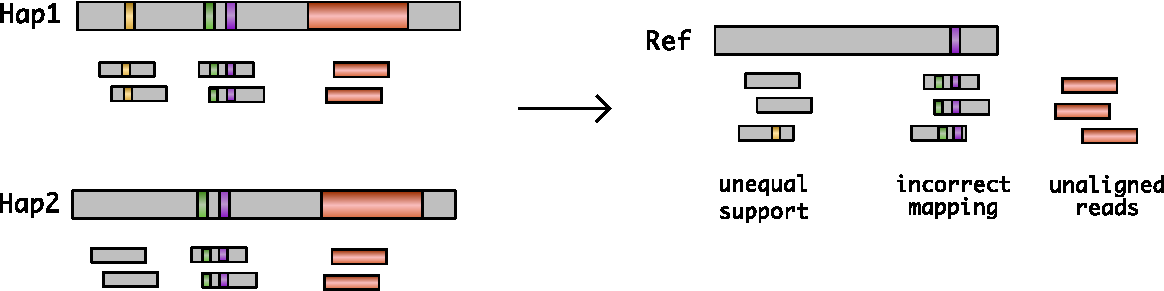
\includegraphics[width=\textwidth]{intro/fig2.pdf}
        \vspace{3mm}
        \caption[Illustration of the reference allele bias]{\textbf{Illustration of the reference allele bias.} \\
        \footnotesize{The origin of short sequencing reads of the sample (hap1 and hap2) are determined by alignments to the reference nucleotides. Thus, the comparison will always be biased towards nucleotides in the reference. Alignment of reads with alleles differing from reference nucleotides might receive lower support than alleles matching to the reference nucleotides (yellow stripe), results in incorrect alignments with multiple variations (green and purple stripes), or remains unmapped if the regions are not present in the reference (e.g., large insertion, purple box). Orange background denotes reference sequences.}}
        \label{fig12:bias}
\end{figure}

\subsection*{The problem of reference bias is pronounced in a species with high genetic diversity}

The effect of reference bias will be more pronounced in a highly diverged species like in cattle. The genetic architecture of the bovine genomes has been shaped by various processes related to domestication, introgression, local adaptation, and human-directed selection \citep{zhang2020evolution}, resulting in the creation of more than 600 subpopulations (known as breeds) adapted for a variety of environmental conditions and selected for various breeding goals. Genetic diversity is higher in cattle than human populations \citep{charlier2016ngs}. The bovine species formed the bovine tribe which subdivided into three sub-tribes diverged about 10-15 million years ago: the \emph{Pseudorygina},\emph{ Bubalina} (Buffalo), and \emph{Bovina} (genus Bison and Bos). Specifically, the subtribe bovina is comprised of three subtribes split about 3-5 million years ago: (i) yak, bison; (ii) gaur,   gayal, and banteng; and (iii) taurine and indicine cattle \citep{pitt2019domestication}. Generally, taurine breeds (\emph{Bos taurus taurus}) are intensively selected for production traits (milk and beef) and have higher fertility than indicine breeds. Indicine breeds (\emph{Bos taurus indicus})  generally have lower production traits and fertility, but still possess desirable traits related to heat tolerance, parasite and disease resistance \citep{Low2020}. However, these characteristics are not strict as there are numerous local cattle breeds optimized for specialized breeding goals \citep{signer2017population,upadhyay2019genomic}. Series of introgressions and hybridizations created specialized breeds with mosaic genomes, such as Brahman, composed of ~10 \% taurine and 90\% indicine origin \citep{koufariotis2018sequencing}. African cattle are generally admixtured between \emph{Bos taurus} x \emph{Bos indicus}, where the introgressed regions are selected for African pastoralism \citep{kim2020mosaic}. On average, each individual cattle carries more than 5 million variants that differ from \emph{Bos taurus} reference, which is higher than reported in the human population \citep{daetwyler2014whole,sudmant2015integrated}. The number of variants is higher in more diverged, indicine \citep{koufariotis2018sequencing} or under-studied African cattle \citep{kim2020mosaic,kim2017genome}. Additionally, this amount likely underestimates the actual genetic diversity as it does not consider structural variations, which are poorly characterized with short-read sequencing technology \citep{mahmoud2019structural,chaisson2019multi}. 

\section{Strategies to mitigate reference bias}

\subsection*{Modification of the existing linear reference genome}

Some strategies have been proposed to mitigate the reference bias. The most straightforward solution is to create a so-called consensus reference genome, whereby each minor allele in the reference sequence is replaced by the most frequent allele in the population. Since the transformed reference is still in the linear space, the downstream genetic analysis can still use the tools currently developed for linear genomes. However, a coordinate lift-over is needed when indels are included in the substitutions. \citet{ballouz2019time} built a consensus human reference by replacing 2 million minor alleles with the corresponding major allele, that reduced mapping error by a factor of three and improved the quantification of transcripts \citep{kaminow2020virtue}. \citet{chen2021reference} extended this idea into a so called reference flow approach, which re-aligns sub-optimally mapped reads into a set of genomes from multiple population, that could reduce strongly heterozygous sites by 22\%. Another effort, as in the human genome, is by continually expanding reference sequences with alternative contigs representing alleles at polymorphic regions that are impossible to assemble with a single haplotype. There were currently 13 updates with 261 alternate patches that add 109 Mb total length. However, this strategy is not sustainable with more diversity included. Additionally, the lack of tools that can properly handle these additional overlapping contigs will likely not be able to mitigate the reference bias and will suffer from increasing mapping ambiguity \citep{sherman2020pan}. 

\subsection*{Creation of population-specific genome assemblies}

The reduced cost of long-read sequencing and improved assembly techniques  make it easier to generate high-quality, near error-free, and near-complete genome assemblies \citep{miga2020telomere,logsdon2021structure}. Thus, more studies have now shifted from species-level references into population-specific reference genomes, effectively creating more personalized genomes. Large genomic initiatives such as the Vertebrate Genome Project (VGP, \url{https://vertebrategenomesproject.org/}) \citep{Rhie2021}, Darwin Tree of Life (\url{https://www.darwintreeoflife.org/}), or Earth Bio-genome Project \citep{lewin2018earth} contribute to the explosion of the number of genome assemblies across the tree of life deposited in the public domain. The first phase of VGP generated 268 vertebrate genomes using long-read data, that were further scaffolded with optical mapping to produce chromosome-scale assemblies fulfilling their strict high-quality criteria \citep{Rhie2021}. On the other hand, some genomic initiatives focus to deeply characterize the diversity of a single species, such as the Human Pangenome Reference Consortium (HPRC) that plans to generate 350 human assemblies representing global ancestries (see \url{https://humanpangenome.org/}). A similar internationally coordinated effort was also initiated for cattle with the Bovine Pangenome Consortium \citep{heaton2021reference} aims at generating generate reference-quality assemblies across global cattle breeds. There are already dozens of genomes from livestock species available in public repositories. As of April 2021, there are chromosome-level assemblies of 22 cattle (\emph{Bos}) and its relatives (gaur, gayal, yak, bison), 19 pigs (\emph{Sus}), 7 sheeps (\emph{Ovis}), 4 goats (\emph{Capra}), 9 dogs (\emph{Canis}), with many more continuing to be added.

\section{Transition from genomics to pangenomics}

\subsection*{Definition of the pangenome}

A pangenome refers to a structure used to  integrate multiple genomes, reflecting the complete species diversity rather than collapsing all variations into a single haplotype, (see recent reviews \citep{bayer2020plant,sherman2020pan,della2021pan}). The term pan-genome (pan – whole, Greek) was first introduced by \citet{tettelin2005genome} to describe complete gene repertoire across \emph{Streptococcus agalactiae} strains where 20\% of the genes are variable across isolates. This concept was quickly adopted across the tree of life, including pig \citep{li2017comprehensive,tian2019building}, goat \citep{li2019towards}, and human \citep{duan2019hupan,sherman2019assembly}. There has been rapid growth in the number of pangenome publications across years \citep{bayer2020plant}, with close to 8000 studies indexed by PubMed,  although most currently focus on bacterial pangenomes.  

\subsection*{Categorization of the pangenome}

The content of a pangenome may be divided into the core and flexible genome (also known  as dispensable or accessory genome, Fig. \ref{fig13:pan}a). The core genome contains sequences common to across all individuals that is responsible for maintaining essential functions (e.g., DNA replication, cellular homeostasis and cellular processes). This part of the genomes is under purifying selection, thus having less diversity. The dispensable genome contains segments that vary across individuals. They are under less evolutionary constraint, which allows for contributions to numerous adaptive phenotypes, mainly disease, biotic, and abiotic resistance, survival, immunity, defence response, adaptation to new environments, communications, and signalling \citep{golicz2020pangenomics}. Thus, dispensable genomes are of particular interest to study adaptive traits that might drive genetic differentiation and give populations their distinguishing characteristics. In mammals, the pangenome is largely dominated by core component (e.g., 96.67\% of genes in the human) \citep{duan2019hupan}. A recent report in the Mediterranean mussel \emph{Mytilus galloprovincialis}, with high-stress tolerance and lineage-specific duplications, indicates that up to 25\% of the total genome is variable \citep{gerdol2020massive}. Pangenomes have been extensively characterized in plants, for instance in rice \citep{zhao2018pan}, tomato \citep{gao2019tomato}, wheat \citep{walkowiak2020multiple}. Plant pangenome seems to have a larger proportion of accessory genomes (>20\%), particularly in polypoid, outcrossing, or species history of whole-genome duplications \citep{tao2019exploring}. Higher ratio of flexible to core genome is typically found in species with higher adaptability \citep{tranchant2018plant}. 

It is important to consider whether the pangenome is of either closed or open type. In a closed type pangenome, the sequencing of sufficient samples will capture the whole pangenome, and thus the size of the complete pangenome can be computationally predicted. On the other hand, sequencing more individuals will recover more pangenome content in an open pangenome. Thus, the size of pangenome keeps increasing as more samples are added \citep{golicz2020pangenomics}. Many plant and animal pangenomes are a closed type in terms of the number of genes but open in terms of total sequence content \citep{duan2019hupan,golicz2020pangenomics}, which also suggests that the non-coding segments primarily drive the sequence variability across individuals. Bacterial pangenomes  are generally open type due to the prevalence of horizontal gene transfer \citep{soucy2015horizontal}. Sampling bias of underrepresented diversity (such as genetically related samples) could lead to the falsely concluding that the pangenome is complete \citep{tranchant2018plant}. With additional, sufficiently  diverged samples, the  pangenome would continue to grow. Thus, the sampling strategy in a pangenome study should maximize diversity to fully retrieve the complete pangenome. 

\begin{figure}[!htb]
    \centering
    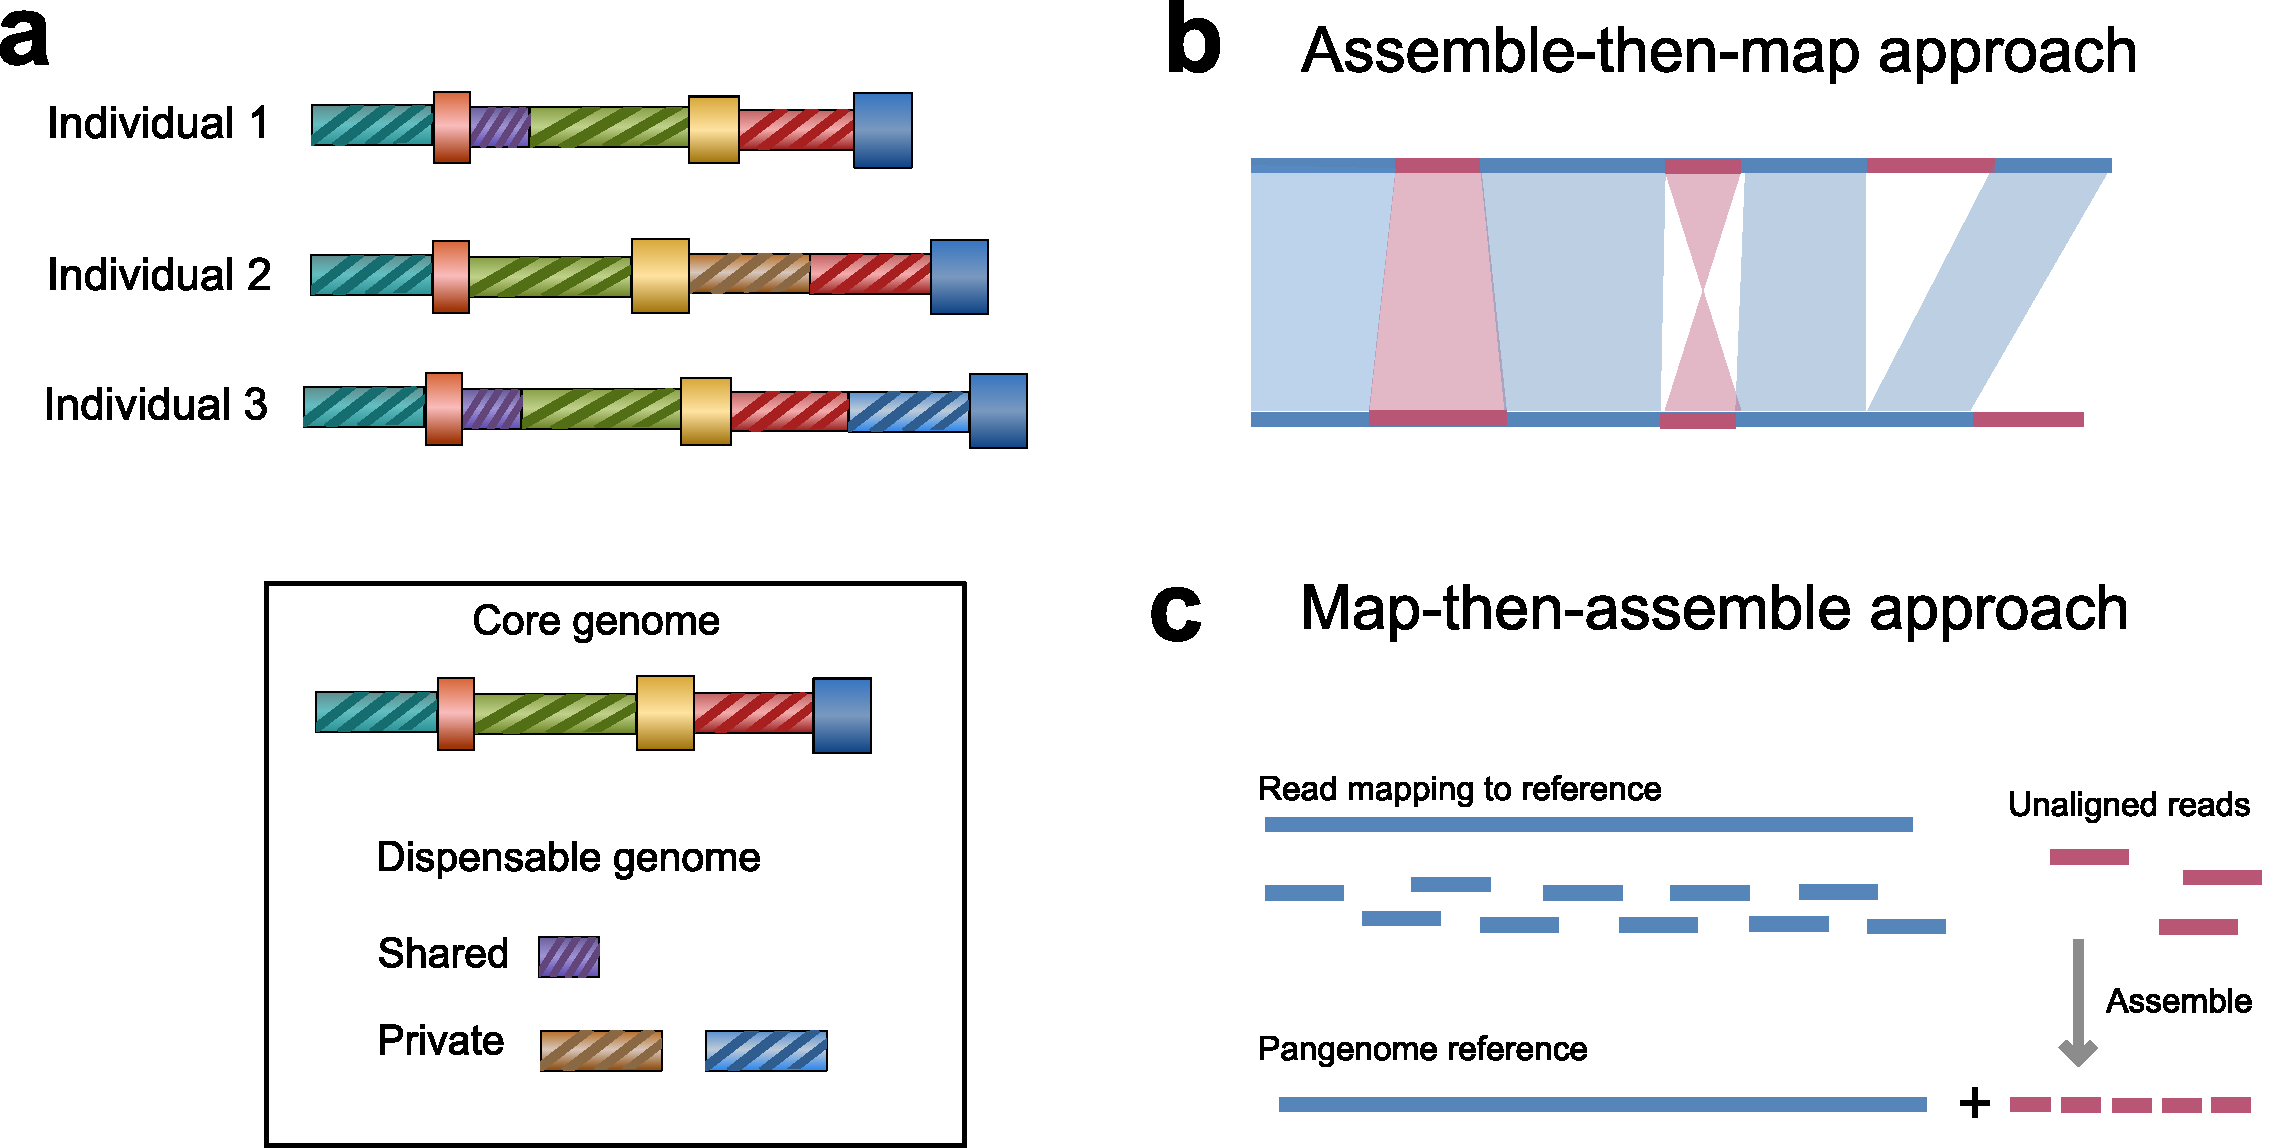
\includegraphics[width=\textwidth]{intro/fig3.pdf}
        \vspace{3mm}
        \caption[The concept of pangenomes]{\textbf{The concept of pangenomes.} \\
        \footnotesize{\textbf{(a)} A pangenome is a collection of individual genomes, which is further divided into core (shared by all individuals) and flexible parts (the presence varies across individuals). Different strategies to build the pangenome: \textbf{(b)} Assemble-then-map: Genomes from multiple individuals are assembled, which are then compared to the reference assembly; \textbf{(c)} Map-then-assemble: sequencing reads from multiple individuals are aligned to the reference. Unmapped sequences are subsequently assembled and added as additional contigs to the reference sequences. Figures are adapted from \citep{sherman2020pan} and \citep{bayer2020plant}.}}
        \label{fig13:pan}
\end{figure}


\subsection*{Approaches to build a pangenome}
% \vspace{-2em}
There are two commonly used approaches to build a pangenome (Fig. \ref{fig13:pan}bc): “assemble-then-map" and “map-then-assemble" (also known as map-to-pan) \citep{golicz2020pangenomics}. In the “assemble-then-map"-strategy, each genome is assembled and annotated independently, which is then followed by pairwise alignment of all assembled genomes to determine shared and non-shared segments \citep{duan2019hupan,li2019towards,eisfeldt2020discovery}. This assembly-based strategy is supposed to recover the full-length non-reference sequences and resolve repetitive and complex structural variants. However, this approach depends on the assembly contiguity and completeness. Assembly and annotation errors make the comparison difficult and may lead to erroneous identification of structural variations. Additionally, genome assemblies are still too expensive to be created at the population-scale, limiting analysis only to a subset of individuals. To take advantage the massive amount of short-read sequencing data, the majority of  recent pangenome studies utilize the “map-then-assemble"-approach \citep{holden2018assembly,laine2019exploring,sherman2019assembly}. Sequencing reads from each sample are independently mapped to the reference genome. The  unmapped (or poorly mapped) reads are subsequently assembled to obtain the non-reference sequences. However, due to the nature of short-read-based assembly, most of the resulting contigs are fragmented, making it difficult to locate the breakpoints (origin) in the reference genome \citep{sherman2019assembly}. 

\section{Graph-based pangenomics}

\subsection*{Graphs as richer reference structures to integrate the genetic diversity}

The pangenome approaches based on unmapped reads or assembly comparison, as discussed above, rely on collections of linear genomes and do not attempt to provide coherent representation that relates all genomes. Considering the prevalence of genetic variations across individuals in the population and abundance of genomic resources, the linear representation is clearly an oversimplification. Emerging pangenome methods are developed to build richer variation-aware reference structures that unify the complete genetic diversity of a species in a non-redundant way. These collective efforts led to a new genomic discipline known as Computational Pangenomics, see review \citep{paten2017genome,computational2018computational,eizenga2020pangenome}.

Graph-based models (also known as genome graphs or sequence graphs) are currently proposed as data structures to unify a collection of related sequences in a compact way (Fig. \ref{fig14:graph}). In a sequence graph, nodes are commonly labelled with sequences and directed edges connect nodes with continuous sequences. Regions without differences are collapsed into a single node allowing compression of redundant sequences. Regions where the samples differ from each other form bubbles, with alternate paths representing different alleles \citep{paten2018superbubbles}. Traversing (or walk through) the graphs recovers the initial input sequences as well as all possible recombinations. \\


\begin{figure}[!htb]
    \centering
    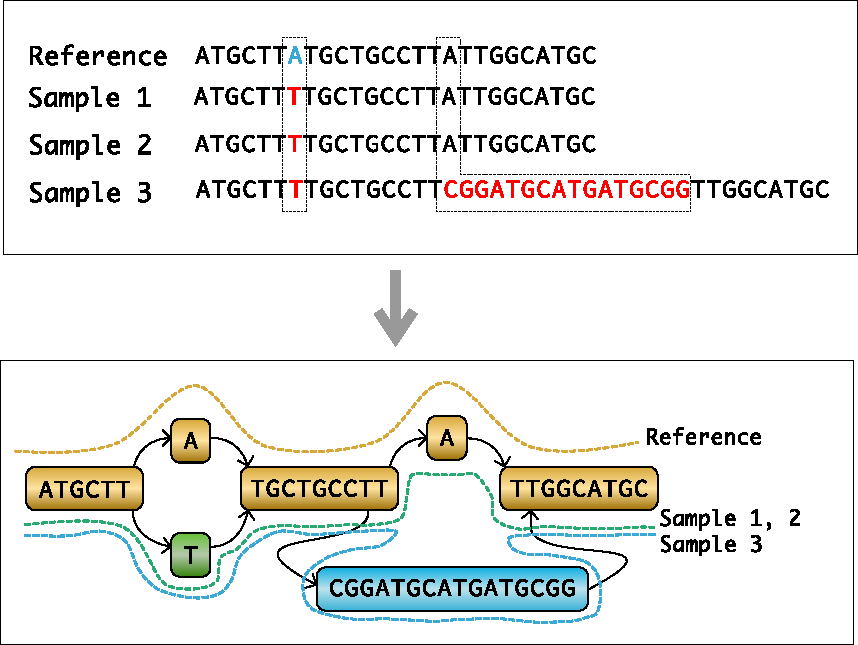
\includegraphics[width=0.8\textwidth]{intro/fig4.pdf}
        \vspace{3mm}
        \caption[Graph-based pangenome approach]{\textbf{Graph-based pangenome approach.} \\
        \footnotesize{\textbf{(a)} Most pangenomes follow the classical pangenome approach, where multiple linear genomes are compared without compressing redundant information and might lack orthologous relationships. \textbf{(b)} A graph-based pangenome approach could unify multiple genomes into a compact and richer reference representation. Nodes contain DNA sequences and nodes with continuous sequences are connected with directed edges. Redundant information across genomes is compacted by collapsing invariant regions into a single node. Alternative nodes in the bubbles (green and blue nodes) are alleles in the population. Thus, graphs allow sequence comparison to occur in the context of variations. Walks through the graph might retrace the original sets of sequences from which it was built (dashed line).}}
        \label{fig14:graph}
\end{figure}


\subsection*{Graph genomes implementations}

The first pangenome graph implementation was based on the DBG (\emph{De Bruijn Graphs}). Sequencing reads from all samples were fragmented into $k$-mer length $k$ (where $k$ < read length), and the graph was constructed by inducing the first and second node where $k-1$ bp end of first node that overlap with the $k-1$ bp start of the second node. Nodes are “coloured” where each colour represents samples. \citet{iqbal2012novo} developed \emph{Cortex}, a coloured DBG-based pangenome tool. They used it to construct a population graph from 164 human samples and identified 3.2 Mb novel sequences that are absent in the human reference genome. Because the genomic coordinates are discarded by fragmenting the reads, DBG-based approaches are not suitable for genetic variant discovery that relies on the reference coordinate, although a recent study attempts to embed a long-range path information into the graph \citep{turner2018integrating}. 

Current well-established graph genome implementations establish a variation graph as an extension of the linear reference genome \citep{eggertsson2017graphtyper,garrison2018variation,sibbesen2018accurate,rakocevic2019fast,kim2019graph}. This implementation utilizes the existing linear reference genome as a backbone, which is then augmented with known variants. To build the graph, reference sequences are split at variable sites, and variants are added as alternative nodes of the reference bases in the graph (Fig. \ref{fig15:vargr}). The linear reference coordinates are embedded in the graphs as a path, and the nodes are referred to relative to this reference path. Thus, the reference path provides a stable coordinate system that can be used as a basis for alignment and annotation \citep{garrison2018variation}. However, large nodes containing sequences not present in the reference genome cannot be represented with the linear genome coordinate, prompting the development of the graph coordinate that directly encode the topology of the graph \citep{paten2017genome,eizenga2020pangenome}. \\


\begin{figure}[!htb]
    \centering
    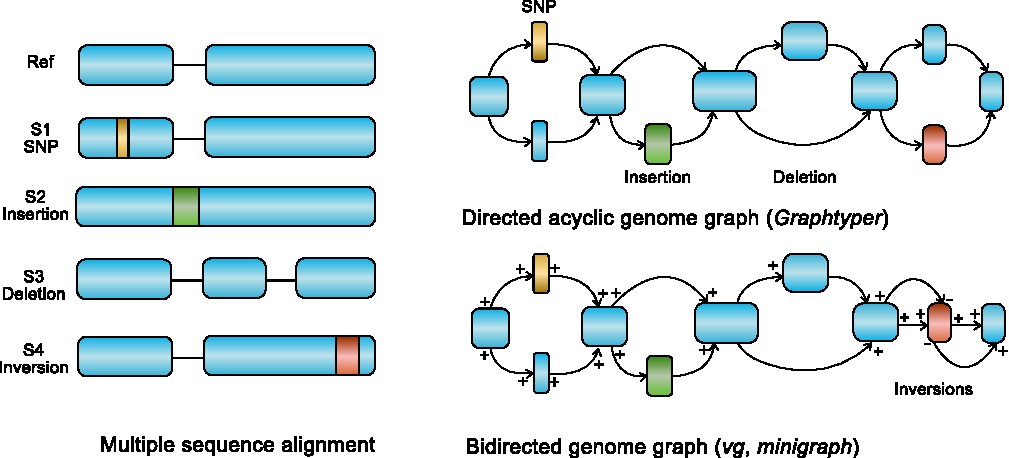
\includegraphics[width=0.8\textwidth]{intro/fig5.pdf}
        \vspace{3mm}
        \caption[Construction of the variation graphs]{\textbf{Construction of the variation graphs} \\
        \footnotesize{A variation graph augments the previously identified genetic variations into a reference sequence backbone as alternative nodes in the graph (green and light blue nodes). Paths that represent the haplotypes of the samples (including reference path) are stored in the graph (coloured lines).}}
        \label{fig15:vargr}
\end{figure}


\emph{Graphtyper }is the first open-source variation graph-based software designed for genotyping from a local (region-specific) graph \citep{eggertsson2017graphtyper,eggertsson2019graphtyper2}. It uses a variant file (\emph{VCF}) as input source of variant sites and a reference assembly as backbone of the graph. Because of the limited variations included in a VCF file, the output graph is directed and acylic containing insertions and deletions but not necessarily complex variations (Fig. \ref{fig16:mut}b). \emph{Graphtyper} applies a two-step genotyping processes. The  “discovery step” is similar to linear reference-guided variant analysis. Sequencing reads are mapped to the linear genome and variants are identified from these alignments. This step is then followed by read realignment towards local graphs. To this end, \emph{Graphtyper} first constructs small regional graphs within 10 kb windows that are subsequently augmented with variants discovered during the first step. Then, \emph{Graphtyper} extracts reads that were initially mapped by the linear mapper, realigns them onto the local graph and performs the variant genotyping from the refined alignments. This approach, however, does not  fully  eliminate reference bias because it relies on the global read placement by a linear mapper. However, this design makes it highly efficient as evidenced with scalable joint genotyping of close to 50,000 human genomes \citep{eggertsson2019graphtyper2}. Additionally, Graphtyper outperformed current state-of-the-art linear genome-based tools (e.g., \emph{SAMtools} and \emph{GATK}), particularly from more refined variants surrounding Indels with considerably reduced Mendelian errors observed in parent-offsprint pairs \citep{eggertsson2017graphtyper}.

\subsection*{Construction of the whole-genome variation graphs with the \emph{vg toolkit}}

The variation-graph toolkit (\emph{vg}) is the first open-source toolkit designed to perform the full suite of genome analyses from genome graphs in species with gigabase-sized genomes \citep{garrison2018variation}. The basic structure of \emph{vg} is a bidirected sequence graph that can express the strand-ness of the input sequences (Fig. \ref{fig16:mut}c). Each edge endpoint has an independent orientation to indicate whether the forward or reverse sequences are spelled out when visiting the node \citep{paten2017genome}. Therefore, \emph{vg} can also represent variations with complex topology e.g., inversions or translocations. An auxilary index is used to store the phasing information so that analysis from the graph can consider haplotypes of the samples \citep{siren2020haplotype}. Graph mapping in \emph{vg} is optimized for short sequencing reads that follows the seed-and-extend paradigm. It relies on a \emph{GCSA2 }graph index (a generalization of linear genome-based\emph{ BWT} index to graphs) for a fast seed query \citep{siren2017indexing}. The index construction is the computationally most demanding step because all $k$-bp paths in the graphs need to be enumerated, which is intractable in complex regions with high variant density. In practice, \emph{vg} can handle complex regions by indexing them on a simplified graph e.g., retaining only biologically plausible paths informed by the haplotype index \citep{siren2017indexing}. Graph mapping is computationally more expensive than linear mapping because multiple alternative paths need to be explored. To make graph-based mapping competitive to linear mapping, \emph{vg mapper} is currently being improved to utilize the minimizer-based mapping paradigm and by restricting the mapping that conforms the haplotype paths. It can achieve the same mapping speed as the \emph{BWA} (linear mapper) with more accurate alignment performance \citep{siren2020genotyping}. 


\begin{figure}[!htb]
    \centering
    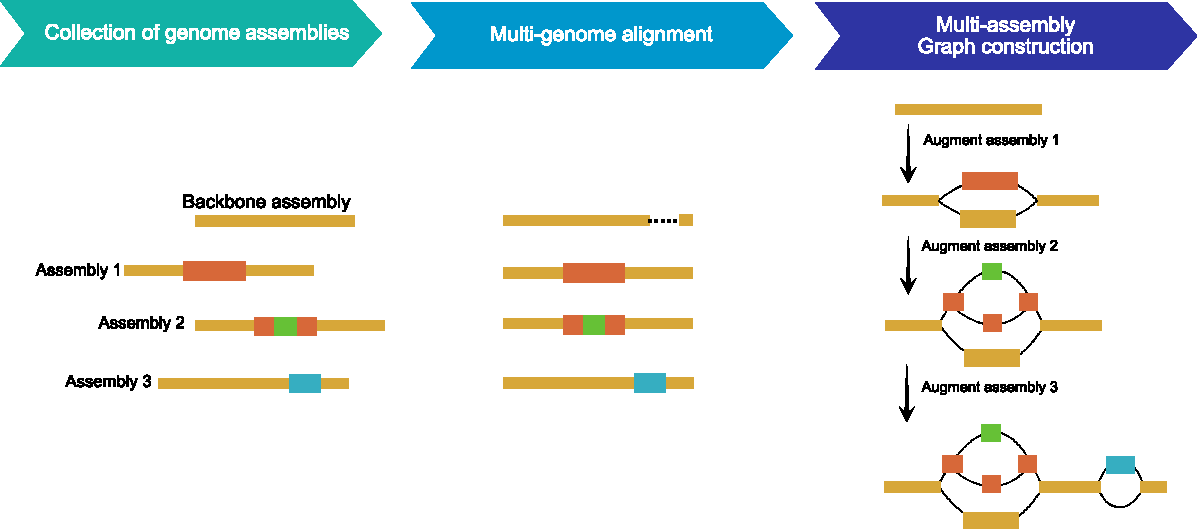
\includegraphics[width=0.9\textwidth]{intro/fig6.pdf}
        \vspace{3mm}
        \caption[Genetic variant representation in the genome graphs]{\textbf{Different genome graph implementations and representations of variations in the graphs} \\
        \footnotesize{\textbf{(a)} multiple sequence alignments capturing sequence relationships. \textbf{(b)} directed genome graphs underlying the data structure of \emph{Graphtyper}; a similar to multiple sequence alignments but with compressing redundant information. \textbf{(c)} general bidirected sequence graph as implemented in \emph{vg} that each edge endpoint has independent orientation. Note  forward (+) and reverse strand (-) to indicate inversions (orange). Figures are adapted from \citet{eizenga2020pangenome}.}}
        \label{fig16:mut}
\end{figure}


\section[Construction of the multi-assembly graphs]{Genome graph construction from a collection of reference-quality assemblies}

\subsection*{Multi-assembly graphs as a framework to integrate multiple genome assemblies}

The construction of graphs by augmenting a reference genome with a predefined set of variants  is still somewhat biased to the reference allele, because the variations are discovered with respect to the reference genome. Additionally, variant identification based on the read alignment is limited by the read length, and thus cannot reliably identify large structural changes between individual genomes \citep{feng2020higher}. Moreover, the input variant file format (VCF) can only model simple variations and is not suitable for representing complex structural variations (e.g., SNPs nested inside long insertions) \citep{letcher2021enabling}.  Building a graph directly from a collection of genome assemblies is a better approach to capture more complete genetic variation. Such a graph will encompass more types of genetic variations, including large structural changes that differ between assemblies (so-called non-reference sequences) that are currently not accessible from linear genomes. This effort will be highly relevant to exploit an ever-increasing number of reference-quality genome assemblies that are being produced at unprecedented rate in order to perform integrative and comprehensive comparative genomics across these resources. 

In the multi-assembly graph approach, graphs are constructed from  multiple whole-genome alignments (Fig. \ref{fig17:multi}). Segments which are present in multiple assemblies without sufficient variation are collapsed into a common node, representing conserved regions or core genomes shared in all input samples. The variable regions form bubbles containing multiple paths of the segments that differ (of poorly or non-aligned sequences) between assemblies. Thus, bubbles in the graph represent structural variations across assemblies, with different paths being different alleles. 

\subsection*{Strategies to build multi-assembly graphs}

Accurate multi-genome alignment is the key for the multi-assembly-based graph approach. However, multiple genome alignment is computationally demanding and scales poorly with the number of genomes. Recently an efficient multiple-genome alignment approach has been implemented in the \emph{Cactus Progressive} software \citep{armstrong2020progressive} that scales to hundreds or even  thousands of genomes while maintaining high alignment accuracy. The key to its computational efficiency and accuracy is dividing a large whole-genome alignment problem into smaller sub-alignment problems using a guide tree. Whole-genome alignment of more than 600 mammals and birds species using \emph{Cactus} enabled a thorough comparative genomics across vertebrate phylogeny \citep{feng2020dense,Genereux2020}.
\citet{hickey2020genotyping} applied the \emph{vg toolkit} to induce graphs from the \emph{Cactus} alignment of 12 yeast strains. Using this approach, they could map more reads with higher mapping quality, mostly due to mapping improvement in the regions harbouring complex structural variations missed from read alignment-based method. 

The approximate mapping between assemblies is another approach to construct multi-assembly graphs. \emph{Minigraph} \citep{li2020design} has recently been developed as a multi-genome graph constructor that extends the minimizer-mapping capability of minimap2 into a graph \citep{li2018minimap2}. It can establish a pangenome graph from 20 human assemblies in under 3 hours with less than 100 GB of memory. The tool applies an incremental graph generation. It uses  a selected genome as a backbone of the graph which is then iteratively augmented with unaligned or poorly mapped segments from the other assemblies. \emph{Minigraph} implemented a hierarchical coordinate system that the sequence coordinate is still retained even with the addition of more assemblies into the graph. Additionally, \emph{Minigraph} simplifies the general bidirected sequence graph data model resulting in a faster and a more straightforward graph analysis. For example, it enforces linearity of the input genomes that produces a graph containing insertions and deletions between genomes but ignoring events that breaks the linearity, such as translocations. Constraining alignment to an anchor genome also ensures that the graphs devoid of highly tangled parts which are difficult to interpet \citep{Lei2021}. Comparative genomics using a pangenome graph built with \emph{minigraph} containing human and its closely related ape species revealed insights into the evolution of repeat-rich regions in primates \citep{li2020design}, which was inaccessible from a linear genome. An unpublished graph pipeline (Pangenome Graph Builder, \url{https://github.com/pangenome/pggb}) aims at building a comprehensive reference-free graph containing all classes of genetic variations with paths that can reconstruct the entire input sequences. However, this method is still in its infancy and requires further testing. \\

\begin{figure}[!htb]
    \centering
    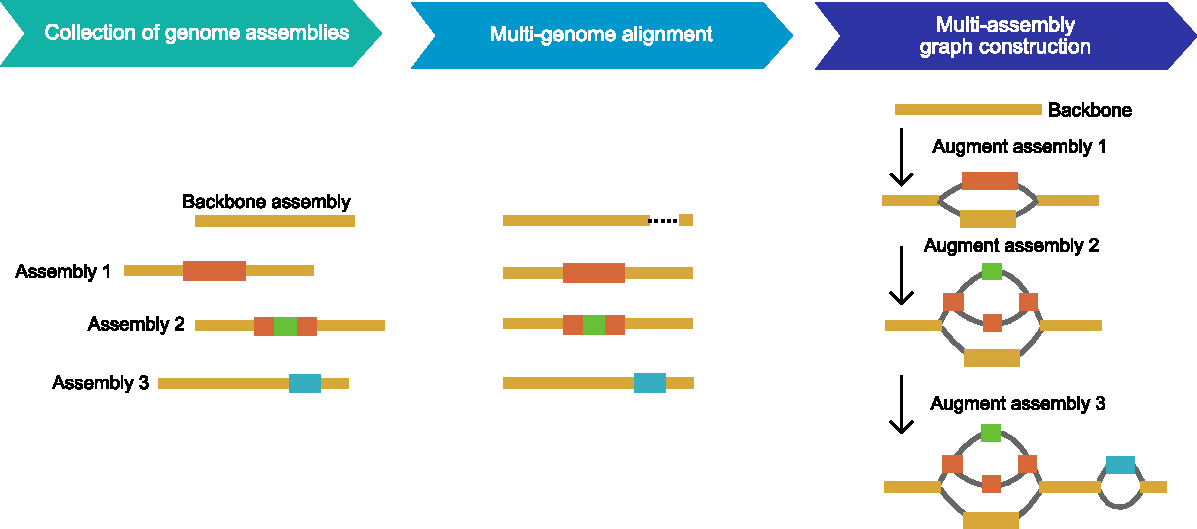
\includegraphics[width=\textwidth]{intro/fig7.pdf}
        \vspace{3mm}
        \caption[Construction of the multi-assembly graphs]{\textbf{Construction of the multi-assembly graphs} \\
        \footnotesize{A multi-assembly graph is built based on multi-genome alignment from the collections of genome assemblies (\emph{left}, \emph{middle}). In the \emph{minigraph} approach (\emph{right}), the graph is built iteratively from alignments of the genome to the backbone or to the existing graph, which is then augmented with diverged sequences from the alignment.}}
        \label{fig17:multi}
\end{figure}

\section[Utilization of the graph genomes]{Utilization of graph genomes for genomic analyses}

Graph genome approaches have been applied to a wide range of genomic analyses, mostly focusing on human or plant genomes. These analyses were initially restricted to challenging regions such as the highly polymorphic Human Leukocyte Antigen (HLA) region \citep{dilthey2015improved,lee2018kourami}, where graph-based methods outperform gold-standard linear genome-based genotyping. Several studies \citep{eggertsson2017graphtyper,garrison2018variation,sibbesen2018accurate,rakocevic2019fast} then assessed the performance of graph-based methods on whole-genome variant discovery and genotyping. For instance, \citet{garrison2018variation} constructed a global human graph that contained 80 million variants catalogued by the 1000 Human Genome Project. They showed that genome graphs enable a considerable improvement in read mapping over linear genomes, particularly for reads that differ from the reference, resulting in substantial reduction in the bias of calling genotypes at large indels. 

\citet{pritt2018forge} estimated that with carefully selected variants, genome graphs could rescue 1.2 million from 30-fold coverage of human whole-genome sequencing data that are incorrectly mapped to the linear reference. \citet{martiniano2019removing} applied the \emph{vg} graph framework to an ancient DNA sample to mitigate reference bias due to short and degraded DNA. The benefit of graph-based mapping translates to substantial improvements in calling indels with sufficient accuracy for population genomic inference. \citet{grytten2019graph} extended \emph{vg} graph capability to analyse ChIP-Seq data. Using a pangenome  of \emph{A. thaliana}, they discovered transcription factor binding sites that are absent in the linear genome. Studying transcription-factor binding motifs from \emph{vg} graphs, \citet{tognon2021grafimo} identified variations in regulatory regions affecting the gene expression that remained undetected from linear genome. 

Graph genomes were also rigorously exploited to investigate large (structural) variations. SV genotyping mainly relies on the indirect inference of abnormal read alignment profiles (such as depth or split mapping) because the alleles are not present in the reference assembly \citep{mahmoud2019structural}. Known structural variants can be reliably  genotyped once included in the graph, even with short-read data, because the sequencing reads can be directly aligned to the corresponding variants. \citet{siren2020haplotype} constructed a \emph{vg} graph from 167 thousand structural variations detected from long-read data across diverse human ancestry. Reanalysis of 5202 short-read sequencing data using this graph considerably improves the SV genotyping. Subsequent analyses led to the identification of thousands of expression quantitative trait loci (eQTLs) driven by these large variations, largely undetectable from the linear reference genome. \citet{liu2020pan}  applied a similar strategy in the recent soybean pangenome. Re-genotyping of 2898 sequenced samples from diverse accessions using a pangenome graph integrated from 26 assemblies enabled the identification of a hitherto unknown 10 kb insertion that is associated with a seed phenotype. 

\section{Applications of the pangenomes}

\subsection*{Pangenome analyses in plant genomes}

Pangenome studies in plants successfully identified a large number of genes not included in the reference and highlight a substantial contribution of large variations to the genetic diversity. For example, a pangenome analysis involving 3000 rice accession identified more than 10,000 genes not included in the reference \citep{wang2018genomic}. A considerable number of non-reference insertions associated with agronomic traits, including seed weight and flowering time, were found from a \emph{Brassica} pangenome constructed from eight long-read-based assemblies \citep{song2020eight}. Interestingly, GWAS signals from these insertions are significantly stronger than the standard SNPs-based association. Using pangenome constructed from 725 tomato accessions, \citet{gao2019tomato} revealed 4873 genes absent from the reference genome and discovered a 2 kb promoter insertion regulating fruit flavour that was lost during domestication. An increasing number of studies shift towards the graph-based approach, which is pioneered by construction of a graph-based soybean pangenome \citep{liu2020pan}. 

\subsection*{Pangenome analyses in human genomes}
% \vspace{-2em}
In human genomics, pangenome analyses following large scale re-sequencing initiatives revealed several important insights. The 1000 Genomes Project revealed that each genome carries more than two-fold regions affected by structural variations (8.9 Mb) than small variations (3.6 Mb) \citep{10002015global}. Importantly, they discovered 240 non-reference genes related to immunoglobulin and glycoprotein with homozygous (knock out) deletions in multiple populations, suggesting their dispensable role \citep{sudmant2015integrated}. Pangenome analyses focusing on the Icelandic population \citep{kehr2017diversity} found a common 766 bp insertion (allele frequency of 0.65) associated with decreased risk of myocardial infarctions. A follow-up study based on 3622 samples sequenced using Nanopore (the largest long-read-based pangenome study to date) found that each Icelandic genome carries on average large insertions covering 10.02 Mb genomic regions and identified a tandem repeat motif strongly associated with height \citep{beyter2020long}. Application of a customized pangenome in Chinese Han population detected 29.5 Mb non-reference sequences, including 185 genes missing from the reference genome \citep{duan2019hupan}. \citet{sherman2019assembly} reported markedly larger non-reference sequences from an African pangenome suggesting the substantial underrepresentation of the African genetic diversity in the current reference genome.

\subsection*{Pangenome analyses in animal genomes}
% \vspace{-2em}
Pangenome approaches have also been applied to livestock and domestic animals, although at a lower rate than in plants or humans. The most notable analysis involves the 44 genomes spanning all extant Ruminant families which revealed insights into evolutionary processes \citep{chen2019large}. \citet{holden2018assembly} identified 4.6 Mb novel insertions from assemblies of non-aligned reads from three dog breeds including  novel insertions at six known disease-associated loci. Analysis of unmapped reads from the reference individual in song bird (\emph{Parus major}), \citet{laine2019exploring} uncovered 1822 genes missing in the reference annotation, including \emph{TRY1}, which is highly expressed in the reference bird. A similar effort to characterize the unmapped reads in the cattle Hereford reference animal discovered a number of parasite genomes which are likely to be associated with the reference animal as a host \citep{whitacre2015s}. 

With a rapid influx of high-quality assemblies, pangenome analysis in animals now transition into the comparison between assemblies. Comparison between Angus (\emph{Bos taurus}) and Brahman (\emph{Bos indicus)} haplotypes-resolved assemblies \citep{Low2020} uncovered an extra copy of \emph{FADS2P1} gene in \emph{Bos indicus}, which is proposed to confer the heat resistance. Analysis of the unaligned sequences between 10 goat assemblies \citep{li2019towards} recovered 38.3 Mb non-reference insertions and identified a large mis-assembled regions in the ARS-1 goat reference genome that includes the prolactin gene region. Analysis of 12 Eurasian pig assemblies retrieved 72.5 Mb novel insertions that are absent in the Duroc-based reference assembly \citep{li2017comprehensive,tian2019building}. Additionally, this study also discovered a non-reference insertion that segregates at high frequency in Chinese breeds (but not in European breeds) encompassing the \emph{TIG3} gene region, which is important for fatty acid metabolism. 


\section{Main knowledge gaps}

A well-annotated reference genome is the foundation for genomic analyses. However, The current \emph{Bos taurus} linear reference genome represents a mosaic haplotype  from a single individual \citep{rosen2020novo}, which poorly represents the cattle diversity across the globe. This inadvertently introduces reference bias when DNA sequences that are diverged from the reference are compared to the reference sequences. A variation-aware, graph-based reference structure, is needed for accurate and unbiased genomic analysis in the cattle population. 

Well-established graph genome methods, implemented in software like \emph{Graphtyper} \citep{eggertsson2017graphtyper} and \emph{vg} \citep{garrison2018variation}, construct graphs by augmenting linear reference backbones with known variants. These graph-based approaches are currently tailored towards human genomics applications and have never been applied  to other gigabase-sized genomes. Large international genomic initiatives, such as the 1000 Bull Genomes Project \citep{hayes20191000}, have provided an exhaustive catalogue of variants segregating across global breeds, prompting the use of these resources to improve genomic analysis in livestock species. Thus, it is appealing to develop genome-graph techniques also in \emph{Bos taurus} to create a variation-aware reference genome. 

Variant prioritization is critical to develop informative graph genomes \citep{pritt2018forge}. Thus, a thorough assessment of factors affecting variant prioritization is required to establish cattle genome graphs. Specifically, it is interesting to investigate whether a unified pangenome graph is as informative as the breed-specific graphs. Due to the unique properties of the subdivided cattle populations, it is feasible to address this question using cattle data. 

Multiple studies \citep{sherman2019assembly,li2017comprehensive,ameur2018novo} have reported that reference genomes may lack of millions of nucleotides with unknown functional relevance. However, this quantity has never been investigated in cattle populations. Multi-assembly graphs now provide a framework to establish the full pangenome of a species. Specifically, with the availability of reference-quality genome assemblies across numerous cattle breeds \citep{rice2020continuous,koren2018novo,rosen2020novo}, a multi-assembly graph may integrate these resources into a unified variation-aware reference structure. Moreover, it is desirable to develop an efficient end-to-end computational pipeline to build comprehensive pangenome graphs and characterize sequence variations in the graphs, which is currently lacking for any livestock population.


\singlespacing
\footnotesize

% uncomment so that references appear on the same page
% \let\Origclearpage\clearpage
% \let\clearpage\relax

% \bibliographystyle{abbrvnat}
\bibliographystyle{unsrtnat}
\bibliography{references/introduction}
%\printbibliography[title=References]

% \let\clearpage\Origclearpage

\ifdefined\BuildingFromMainFile
\else
   \end{document}
\fi